\section{Introduction}

\begin{frame}
	\frametitle{Challenging Problem}
	
	\begin{center}
		\begin{tikzpicture}
			\node at (0,0) [draw=white,ultra thick,inner sep=0pt]
			{
				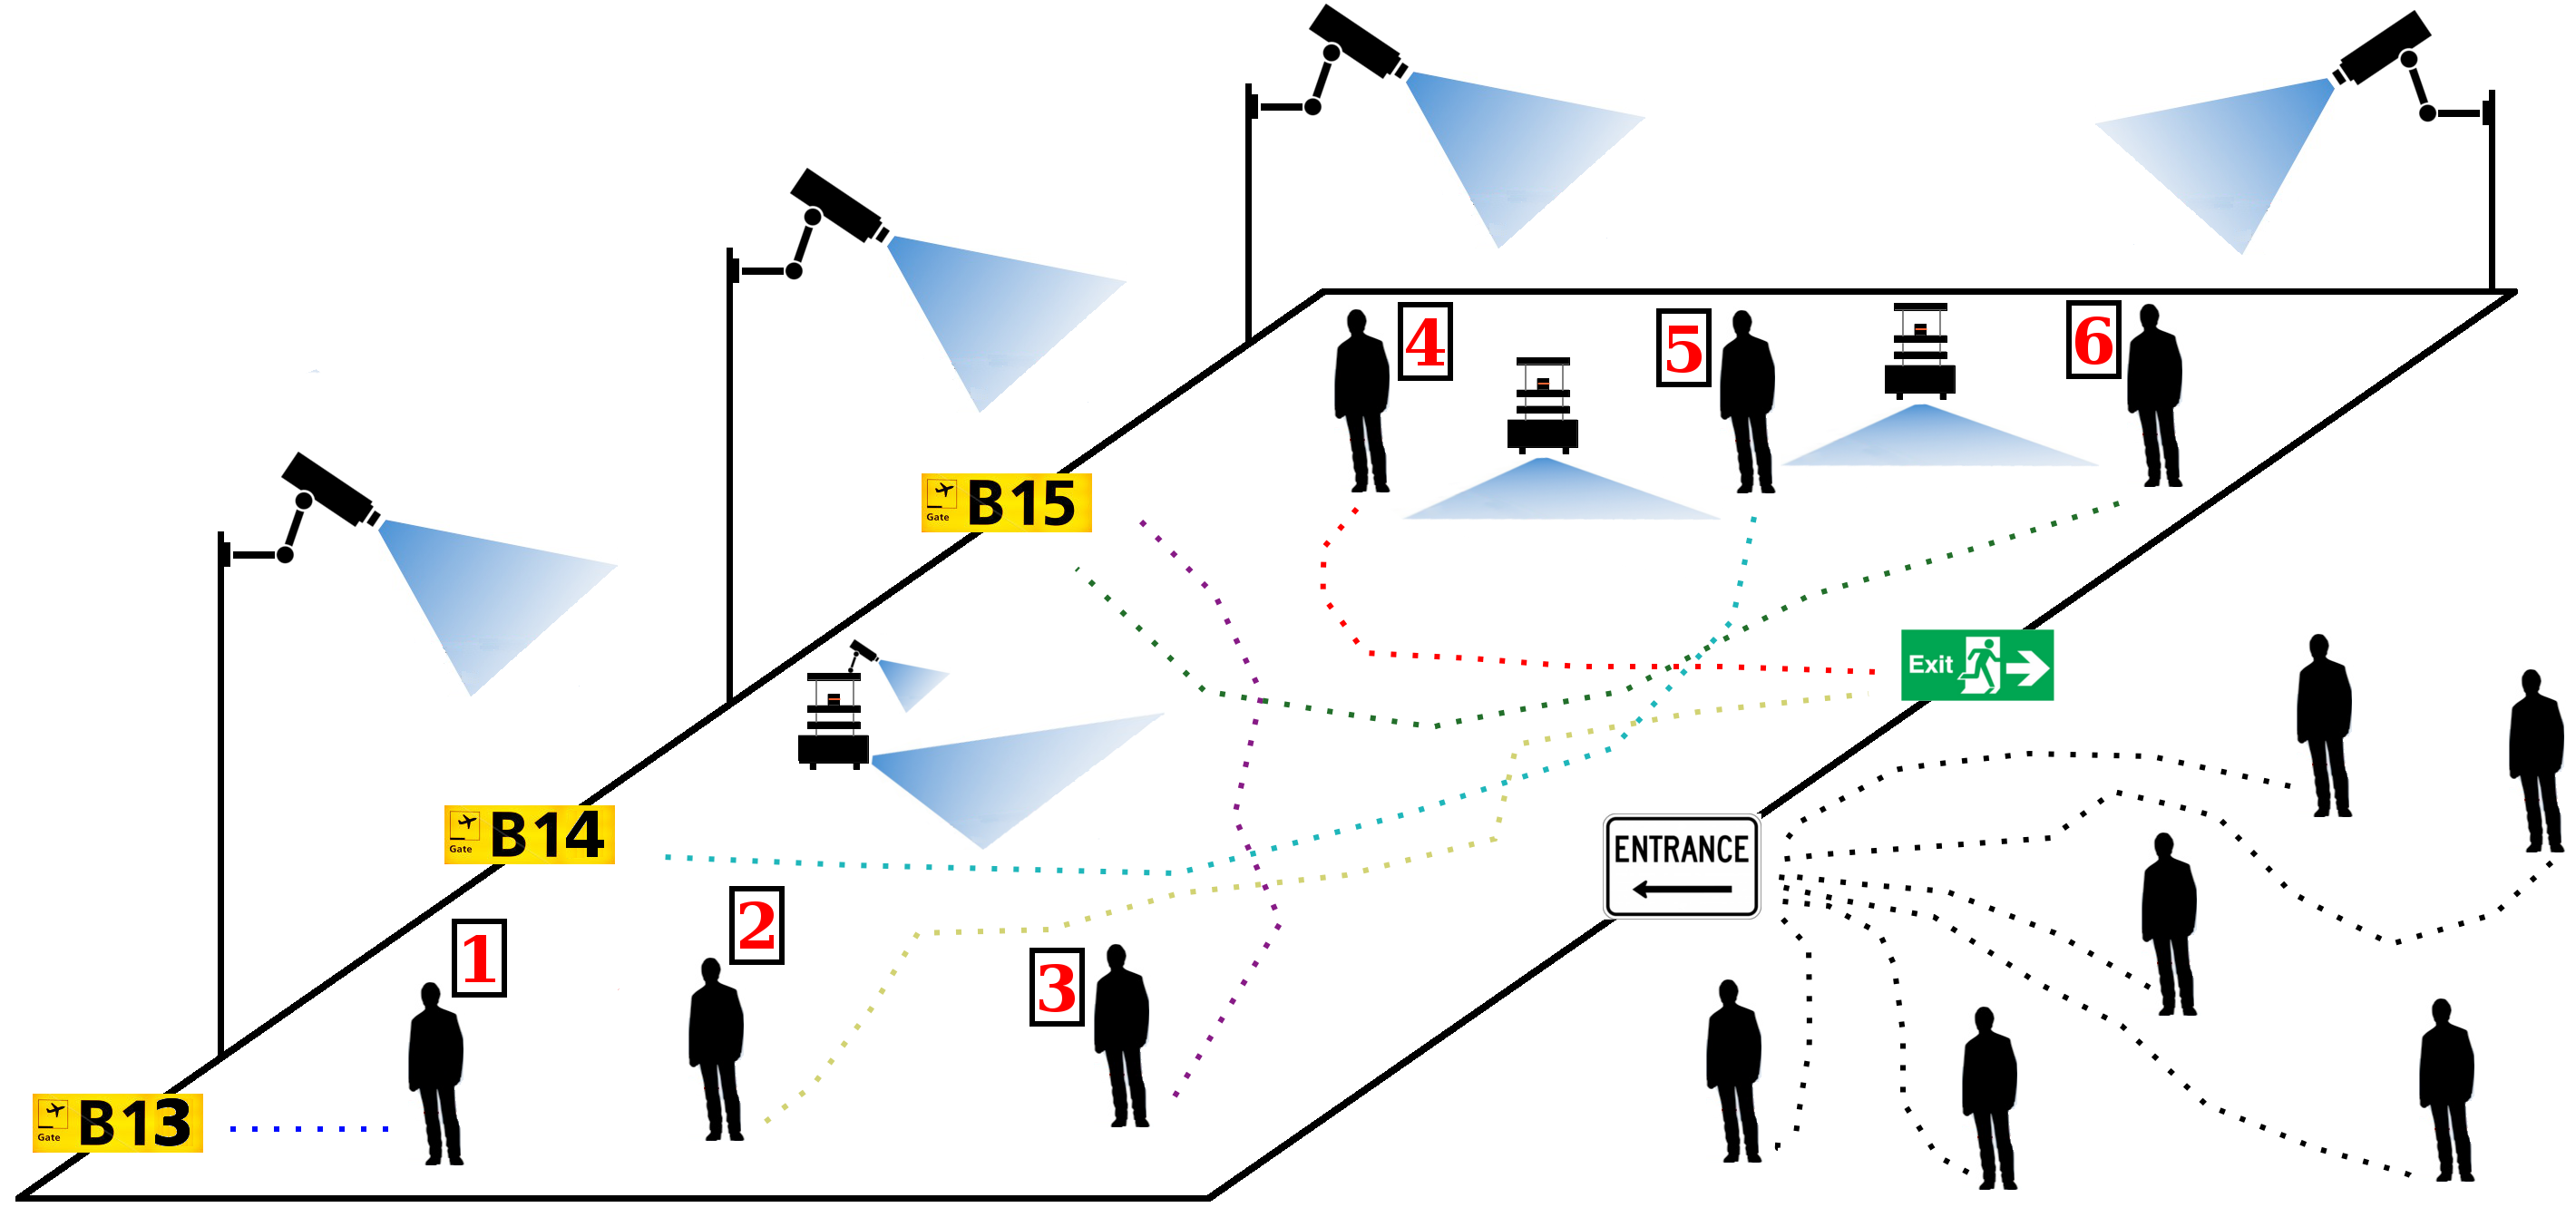
\includegraphics[width=\linewidth]{Figures/Problem.png}
			};
		\end{tikzpicture}
	\end{center}
\end{frame}

\begin{frame}
	\frametitle{Motivation}
	
	\vspace{0.2cm}
	
	\Large
	
	\begin{block}{Objective}
		\textbf{Understanding} the concept of human preference \textbf{allows} to perform higher levels
		of reasoning about future human actions. Likewise, the \textbf{knowledge} of a goal also gives
		information about \textbf{what} a person might do
	\end{block}
	
	\vspace{0.3cm}
	
	Example of application fields:
	\begin{itemize}
		\item Automatic video surveillance
		\item Human-Robot Interaction
		\item Domestic robots
	\end{itemize}
\end{frame}

\begin{frame}
	\frametitle{Contributions}
	
	\Large
	
	\begin{enumerate}
		\item \textbf{Distributed real-time} multiple object tracking, \textbf{asynchronous} and
			  \textbf{fully} scalable design\footnote{\tiny Previtali \emph{et
			  al.}, ``PTracking: Distributed Multi-Agent Multi-Object Tracking through Multi-Clustered
			  Particle Filtering'',\\ \hspace{2.02cm} International Conference on Multisensor Fusion and
			  Integration \\ \hspace{0.5cm} Previtali \emph{et al.}, ``Multi-Robot Surveillance through
			  a Distributed Sensor Network'', Studies in Computational Intelligence}
		\item \textbf{Prediction} without prior semantic scene knowledge and \textbf{incremental}
			  updates of the \emph{IRL} model over time using \textbf{non uniform grids} for
			  representing the state\footnote{\tiny Previtali \emph{et al.}, ``IRL-based Prediction of
			  Goals for Dynamic Environments'', Machine Learning for Social Robotics at ICRA\\
			  \hspace{0.5cm} Previtali \emph{et al.}, ``Predicting Future Agent Motions for Dynamic
			  Environments'', IEEE/RSJ International Conference on\\ \hspace{2.02cm} Intelligent Robots
			  and Systems [submitted]}
		\item \textbf{Efficient} and \textbf{scalable} solution for on-robot deploy\footnote{\tiny
			  Previtali \emph{et al.}, ``Counterfactual Reasoning about Intent for Interactive
			  Navigation in Dynamic'', IEEE/RSJ International\\ \hspace{2.02cm} Conference on
			  Intelligent Robots and Systems\\ \hspace{0.5cm} Bordallo \emph{et al.},
			  ``Interactive Costmaps: Integrating Prediction and Planning with Counterfactual
			  Reasoning'', IEEE/RSJ\\ \hspace{2.02cm} International Conference on Intelligent Robots and
			  Systems [submitted]}
	\end{enumerate}
\end{frame}

\begin{frame}
	\frametitle{Proposed Solution}
	
	\vspace{0.5cm}
	
	\begin{tikzpicture}
		\node at (0,0) [draw=white,ultra thick,inner sep=0pt]
		{
			\includegraphics[width=\linewidth]{Figures/Architecture}
		};
	\end{tikzpicture}
\end{frame}
